
\chapter{Device 1: prototype for spatio-angular illumination}
\begin{summary}
   - Im vorhergehende Kapitel haben wir das dem spatio-angularen
     Mikroskop zugrundliegende Konzept dargestellt. Hier gehen wir auf
     zusaetzliche Details ein, die fuer die praktische Implementierung
     wichtig sind. Unter anderem die Eigenschaften der beiden
     verwendeten Displays, elektronische Synchronisation der
     verschiedenen Komponenten und einem Algorithmus, um das             % /Hier mehr spezifische Probleme/
     Koordinatensystem der Kamerapixel und der Pixel des focal plane
     SLM ineinander zu transformieren.

   - Das pupil plane SLM wurde durch unseren Partner Fraunhofer IPMS
     waehrend des Projekts neu entwickelt.  Daher widmen wir uns diesem   % /MMA kommt spaeter extra/
     Subsystem im Kapitel (FIXME) naeher.
\end{summary}
\section{Description of the optical components}
So far we have only shown the beam path for transmissive displays (in
\figref{fig:memi-simple}). Such SLM only have a very low transmission
in practice. Therefore we use reflective displays in our prototype.

In \figref{fig:memi-real} I adjusted the beam path accordingly. This
schematic also depicts the optics we use to adapt light from the laser
to fill the etendue of our system. The light source enters the system
from the bottom left. The optic components are color corrected and
have anti-reflex coating for wavelengths in the range from
\unit[400]{nm} to \unit[700]{nm}.

The system successively illuminates the pupil plane SLM---a grayscale
micromirror array developed by our project partner Fraunhofer IPMS
Dresden---and the focal plane SLM, a commercial binary liquid crystal
on silicon display.
 
I gathered some of the following details from the documents that were
created during the development of our prototype and are classified as
confidential. I have summarized the key decisions here and the
relevant project partners have agreed to the publication (FIXME not
finished).


\begin{figure}[!htbp]
  \centering
  \svginput{2}{memi-real}
  \caption{Schematic of the light path through our microscope. Laser
    light enters from the lower left, is scrambled and homogenized to
    illuminate the pupil plane SLM in P'' and the focal plane SLM in
    F'. $F$ is the field plane in the sample and its primed versions
    are conjugated planes. $P$ is the pupil of the objective. $B_0$
    and $B_1$ are adjustable circular apertures. PBS is a polarizing
    beam splitter. DBS is a dichromatic beam splitter.  The red boxes
    deliminate subsystems of the illumination system: {\bf A:} light
    scrambling and homogenization, {\bf B:} Fourier-optical filter to
    provide intensity modulating pupil plane SLM. {\bf C:}
    Polarization based intensity modulator as focal plane SLM. {\bf
      D:} Wide-field fluorescence microscope with detection
    path. (FIXME finish diagram, don't use B twice)}
  \label{fig:memi-real}
\end{figure}

\subsection{Ensuring homogeneous illumination}
A quantitative evaluation of our experiments (FIXME ref sec:results)
with different illumination patterns is simplified when both pupil
plane SLM and focal plane SLM are uniformly illuminated.

We use either a laser\footnote{Lasever LSR473H, diode-pumped solid
  state laser, output power 600mW, $\lambda=\unit[473]{nm}$} or an
light emitting diode (LED) \nomenclature{LED}{light emitting diode} as
the light source in our experiments. Below we discuss optical measures
that attain homogeneity of the illumination of both displays.

The LED\footnote{Huey Jann HPB8-48KBD, wavelength
  $\unit[(463\pm1)]{nm}$, brightness \unit[35]{lm}, view angle
  $120{}^\circ$, FIXME TODO: Flaeche messen} we use has a large active
area. Due to etendue mismatch a relatively large amount of its
produced light will never reach the sample. But it is easy to achieve
a homogeneous illumination. Moreover, the LED can be quickly switched
on and off electronically \footnote{The DPSS Laser doesn't allow fast
  direct electronic switching at full power. We have to use an
  acousto-optic modulator connected with the additional expense of its
  optical alignment (FIXME siehe spaetere ref section).}.

Unlike an LED, a laser delivers light of considerably higher spectral
radiance ($\unit[]{W/(sr\, m^2 m)}$). Thus it is in principle possible
to use the laser as a highly efficient light source for our
system. Unfortunately, the high spectral and spatial coherence of a
laser often lead to high-contrast fluctuations of the irradiance and
we have to compensate for this by time averaging.

When using the Laser, we send its parallel Gaussian beam into a
bundle\footnote{Fiber bundle with circular cross-section,
  \unit[1.1]{mm} diameter and \unit[2]{m} length. The beam broadening
  is $3{}^\circ$ and increases, when the bundle is bended
  (\cite{D8.4}).} of randomly distributed fibers (Loptec, Berlin,
DE). This gives a randomized light distribution at the bundle output.

A relay system (A1) images the circular output of the fiber bundle
onto the entrance of a light pipe. This relay system contains a
rotating microlens array\footnote{pitch \unit[0.5]{mm}, focal length
  \unit[23.5]{mm}, beam broadening $\pm 0.23^\circ$ (FIXME erhard
  fragen)}. It mixes the light by illuminating the specimen with many
different mode profiles during one exposure of the camera.

Inside of the hollow mirror-integrator tunnel (see
\figref{fig:integrator-rod}) of quadratic cross-section
\footnote{priv. comm.  Herbert Gross: ``A light guide homogenizes the
  light when its cross section can be put together to cover a plane.''}
the light is mixed by multiple reflections. The light distribution at
the tunnels output is made more uniform without altering its numerical
aperture.




 - Durch mehrfache Reflexion im Lichttunnel (hollow
   mirror-integratortunnel, quadratische 2.5mmx2.5mm cross section,  % /Laser homogenisieren/ 
   250mm laenge, siehe Bild 4.2)  wird das Licht
   zu einer homogenen Lichtverteilung gemischt, ohne die numerische
   Apertur zu aendern (FIXME ref dlpa022.pdf).  Eine Relais-Optik (A1
   und A2 in Fig 4.1) vergroessert\footnote{Ein Tunnel mit $\unit[4\times4]{mm^2}$
   Querschnitt beduerfte nicht dieser Optik, dann waeren die Winkel
   der Strahlen im System jedoch noch kleiner und der Tunnel muesste
   unhandlich lange werden.} 
   den Tunnelausgang des Tunnels auf $\unit[4\times4]{mm^2}$
   in die Ebene F'''.

   \jpginput{8cm}{integrator-rod}{Hollow mirror-integrator tunnel with
     a quadratic cross section of \unit[2.5]{mm}
     side length and \unit[250]{mm} length.}



 - Zu den zwei Relais-Systemen hat der Optikdesigner kommentiert
   (FIXME ref D8.9), dass diese nicht fuer eine perfekte Abbildung,
   sondern fuer einen guten Transport der homogenenen Lichtverteilung    % /Interessantes zu Relais-Systemen an Tunnelenden/
   optimiert wurden. Beim System A1 am Tunneleingang werden drei Elemente
   (FIXME oder 2?, und wo ist das Mikrolinsenarray) eingesetzt, um das
   Licht vom runden Faserende in den quadratischen Tunneleingang zu
   transportieren. Am anderen Ende (A2 Fig 4.1) transportieren fuenf Elemente das
   Licht vom Tunnelausgang in die Ebene F''' mit der
   Beleuchtungsapertur.

 - Waehrend der Konzeption wurde auch eine auf zwei Mikrolinsenarrays    % /Nicht benutzt alternative/
   (fly's eye condensor) basierende Optik fuer die Homogenisierung des Lasers in
   Betracht gezogen (FIXME ref D8.2). In-Visions Planung zufolge,
   waere dieser jedoch schwieriger zu justieren als der Tunnel und
   zudem nicht fuer den vollen Wellenlaengenbereich von 400 bis 700nm
   verwendbar gewesen.

  - Um eine homogene Ausleuchtung mit dem Tunnel zu erreichen sind       % /Erfahrungen/
    folgende Punkte wichtig (FIXME ref D8.5):

   - Das Buendelende sollte den Tunneleingang deutlich ueberdecken. Es
     muss vermieden werden, dass die Tunnelecken dunkler als die Mitte
     des Tunnels sind. Ein inhomogen ausgeleuchteter Buendeleingang
     fuehrt zu inhomogener Beleuchtung des pupil plane SLM.

   - Das Ende des Faserbuendels muss in vier Achsen justiert werden
     koennen (Zentrierung von Position und Winkel).

   - Die Brennweite der Mikrolinsen sollte kuerzer gewaehlt werden,
     als die Rechnung vorhersagt. Damit kann unweigerlich auftretendes
     Mikrochipping der zementierten Glasspiegel kompensiert werden.

\subsection{ Fourier-optischer Filter zur Kontrasterzeugung am pupil plane SLM}
  - Der micro-mirror array, den wir als pupil plane SLM einsetzen,        % /MMA torsion spiegel/
    besteht aus Torsionsspiegeln, die die Phase des Lichts modulieren
    (fuer eine genauere Beschreibung siehe spaeteres Kapitel               
    FIXME). Um damit eine Intensitaetsmodulation zu bewirken, nutzen
    wir den in Fig 4.2 B gezeigten Fourier filter. 

  - Die Linse L1 hat zwei Aufgaben: Zum einen bildet sie die Feldmaske   % /Schlierenoptiklinse/
    B0 in den Feldstopp B1 ab. Zum anderen wird die Ebene P'' mit dem
    SLM nach unendlich abgebildet.

  - Bei ungekippten Spiegeln, wird somit F''' nach F'' abgebildet und    % /MMA Kontrasterzeugung/
    gleichzeitig gibt es ein scharfes Bild von P'' nach P'. Beide
    Ebenen F'' und P' sind dann homogen ausgeleuchtet.

  - Werden die Spiegel auf der linken Haelfte in P'' gekippt, dann
    lenken sie das Licht entlang der gestrichelten Linie (in Fig 4.1)
    ab. Dieses Licht wird von der Apertur B1 absorbiert und steht dann
    nicht in P' zur verfuegung. D.h. die rechte Seite in P' ist
    dunkel. Der gesamte radiant flux ($\unit[]{W}$) durch die Apertur in
    F'' nimmt ab, die irradiance ($\unit[]{W/m^2}$) ueber die Apertur
    bleibt aber homogen.

  - Im realen System besteht die Linse L1 aus 4 Elementen. Aufgrund
    der Symmetrie weist sie keinen axialen Farbfehler auf. Es bleibt
    jedoch ein kleiner lateraler Farbfehler (FIXME genauer ergruenden
    was das bedeutet).
 

\subsection{ Relais-System zwischen pupil plane und focal plane SLM}
  - Die Linsen L2 und L3 bilden ein doppelt telezentrisches             % /Relais-System/
    Relais-System mit Vergroesserung 2 und bilden F'' auf der Ebene
    des focal plane SLM in F' ab. Gleichzeitig bildet dieses
    Relais-System den pupil plane SLM von P'' nach unendlich ab.
 
  - Prinzipiell koennte man auch den focal plane SLM in F'' an Stelle
    der Apertur B1 platzieren. In unserem Prototypen haben wir uns
    jedoch fuer dieses zusaetzliche Relais-System entschieden, um den
    Kontrast beider SLM voneinander zu entkoppeln.

   - TODO warum haben wir das relay system? 
     - vermutlich weil wir den mma kontrast vom lcos entkoppeln wollen
     - es ist natuerlich fuer sammelnde system, dass axial color sich
       aufaddiert und nicht kompensiert wird


\subsection{ Polarisationsbasierte Kontrasterzeugung am focal plane SLM}
  - Der von uns verwendete focal plane SLM ist ein liquid crystal on
    silicon Geraet, dass die Polarisation des reflektierten Lichts
    entweder um 90 grad dreht oder konstant laesst.
 
  - Ein Polarisationsstrahlteiler erzeugt daraus einen binaeren
    Intensitaetskontrast (siehe Fig 4.1 C).

  - Wir haben uns fuer einen wire-grid Polarizer (Moxtek PBF02C, Orem,
    UT, US) entschieden, weil die Platte weniger Rueckreflexe
    verursacht als ein Strahlteilerwuerfel.

  - Die s-Polarisation des eingehenden Lichts wird in Richtung des SLM
    reflektiert. Aktive Pixel des SLM rotieren die Polarisation des
    Lichts um 90 Grad und passiert dann den Strahlteiler als
    p-Polarisation in Tranmission in richtung Mikroskop. Dort befindet
    sich ein zusaetzlicher Cleanup-Analysator im Strahlengang.
 
  - Es waere auch denkbar, SLM und Strahlteiler anders anzuordnen, so
    dass das vom SLM kommende Licht in das Mikroskop
    \emph{reflektiert} wird. In diesem Fall verschlechtert jedoch eine
    ungewollte Oberflaechendurchbiegung des Strahlteilers die
    Abbildungsqualitaet vom focal plane SLM. Deshalb nutzen wir den
    Strahlteiler in Tranmission.

  - Die duenne Platte (<2mm) des Strahlteilers macht das System leicht
    asymmetrisch und fuehrt damit hauptsaechlich zu Astigmatismus und
    lateral color (ref D8.9 FIXME), das Optikdesign bleibt aber
    beugungsbegrenzt.


\jpginput{14cm}{setup-photo-blueprint}{The wide field epi-fluorescence
  microscope with attached illumination head. The positions of the two
  spatial light modulators (Micro mirror array (MMA) and liquid
  crystal on silicon display (LCoS)) are indicated. Drawing by Josef
  Wenisch (In-Vision, Austria).}


\jpginput{14cm}{memi-setup-only-lenses}{only lenses7}

\subsection{ Variables Teleskop als Tubuslinse}
  - Die groesse der Pupille von Mikroskopobjektiven haengt von deren
    Bildfeld und numerischer Apertur ab. Die letzt Linse
    TL${}_\textrm{ill}$ in unserem Beleuchtungssystem ist daher so
    konzipiert, dass sie P'' mit variabler Vergroesserung nach P
    abbildet. 

  - Die Linse besteht aus drei beweglichen Gruppen und kann somit
    garantieren, dass der pupil plane SLM bei Vergroesserungsaenderung
    stationaer auf der pupil plane des Objektivs abgebildet bleibt und
    gleichfalls der focal plane SLM immer im unendlichen abgebildet
    bleibt (FIXME gibt es ein paper mit begruendung?).





\begin{figure}[!htbp]
   \centering
   \svginput{2}{memi-sketch}
   \caption{Schematic of the lenses in the MEMI system and their focal
     lengths. The focal length $f_\textrm{TL}$ of the tube lens can be
     varied. This allows to scale the second intermediate image
     $r''_\textrm{MMA}$ of the micro mirror array to fit the back
     focal plane of different objectives. Dimensions in mm.}
   \label{fig:memi-sketch}
 \end{figure}




% \imagw{14cm}{mma}{{\bf left:} Scanning electron microscope image of
%   the micro-mirror array (MMA).  The pixel pitch of the device is
%   \unit[0.016]{mm}. The hinges for the tilt movement and the
%   electrodes are clearly visible. {\bf middle:} Optical reflective
%   microscope image of the MMA. {\bf right:} exaggerated rendering of
%   how a 8x8 checker board pattern would be displayed on the
%   device. Electron and optical micrograph by Fraunhofer IPMS Dresden
%   (Germany)}

% \begin{figure}[!hbt]
%   \centering
%   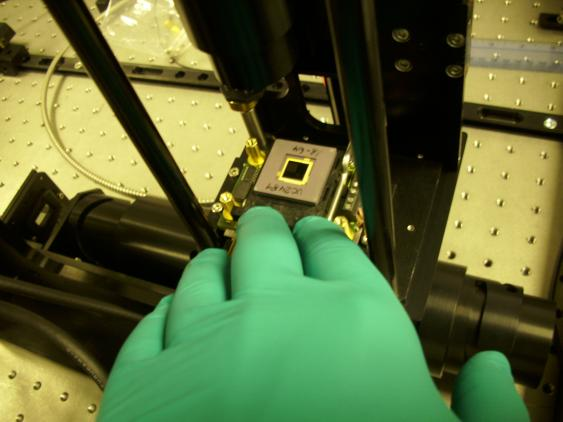
\includegraphics[width=7cm]{mma-plain}
%   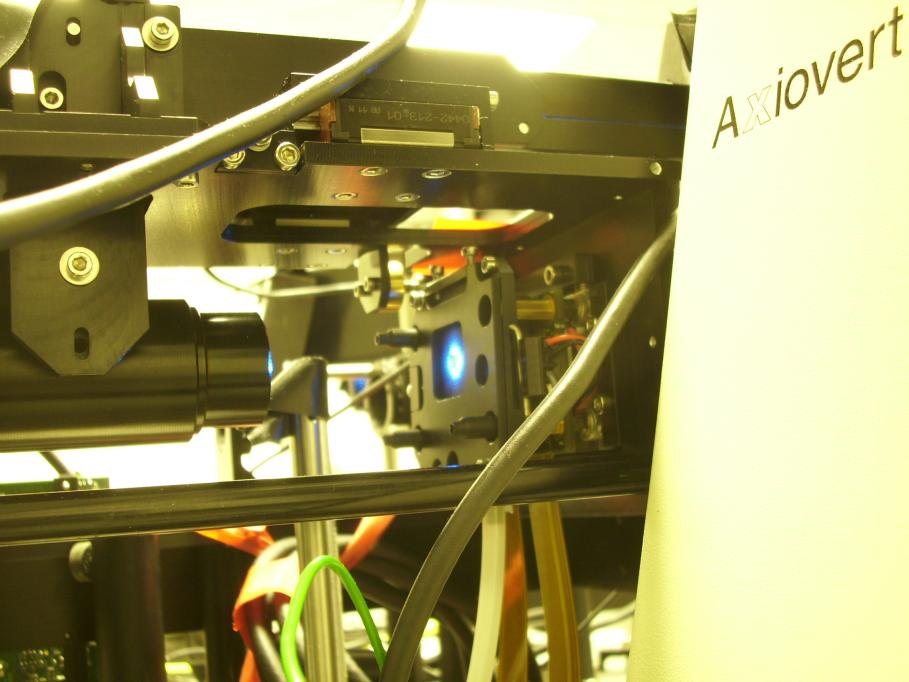
\includegraphics[width=7cm]{mma-ill}
%   \caption{{\bf left:} Micro mirror array chip during installation of
%     the optics. {\bf right:}~Illuminated micro mirror array in the
%     aligned system.}
%   \label{fig:mma-closeup}
% \end{figure}
